\documentclass[pdftex,12pt,a4paper]{report}

\usepackage[portuguese,english]{babel}
\usepackage[T1]{fontenc} 
\usepackage[utf8]{inputenc}
\usepackage[pdftex]{graphicx}
\usepackage{minitoc}
\usepackage{hyperref}
\usepackage{indentfirst}
\usepackage[compact]{titlesec}
\usepackage{fancyhdr}
\usepackage{caption}
\usepackage{pgfplots}
\usepackage{pgfplotstable}
\usepackage{fixltx2e}
\usepackage{mathtools}
\usepackage{fancyhdr}

\pagestyle{fancy}
\renewcommand*\thesection{\thechapter\arabic{section}}
\newcommand{\HRule}{\rule{\linewidth}{0.5mm}}
\begin{document}

\begin{titlepage}

\begin{center}


\includegraphics[width=0.15\textwidth]{./logo}\\[0.5cm]    

\textsc{\large Universidade de Aveiro \\[1cm]\large departamento de electrónica, telecomunicações e informática}\\[1cm]

\textsc{\large{47023}\large - Arquitectura de Redes \\[1cm]}

\HRule \\[0.5cm]
{ \large \bfseries Projecto de Redes}\\[0.4cm]
\HRule \\[1cm]

\textsc{\small{8240 - MESTRADO INTEGRADO EM ENGENHARIA DE COMPUTADORES E TELEMÁTICA}}\\[1cm]

\begin{minipage}{0.4\textwidth}

\begin{flushleft} \large
\href{mailto:rafael.ferreira@ua.pt}{António Rafael da \\ Costa Ferreira }
 \small{\\NMec: 67405 | P4G1}
\end{flushleft}
\end{minipage}
\begin{minipage}{0.4\textwidth}

\begin{flushright} \large
\href{mailto:rodrigocunha@ua.pt}{Rodrigo Lopes \\ da Cunha}
\small{\\NMec: 67800 | P4G1}
\end{flushright}
\end{minipage}\\[1cm]

{\large Docente: António Manuel Duarte Nogueira  }\\[0.5cm]

\vfill

{\large Junho de 2015 \\ 2014-2015}

\end{center}

\end{titlepage} %Titulo do Relatorio
\renewcommand{\headrulewidth}{0pt}

%Cabeçalhos de rodapé
\fancyhead{}
\fancyfoot{}
\lhead{Football Club - Trabalho Prático Final}
\rhead{BD - 2014/2015}
\lfoot{\textit{P4G1} \\ Rafael Ferreira nmec: 67405 \\ Rodrigo Cunha nmec: 67800}
\rfoot{\thepage}

%Renomear Comandos
\renewcommand*\contentsname{Conteúdos}
\renewcommand*\figurename{Figura}
\renewcommand*\tablename{Tabela}

%Conteúdos, dar paragrafo
\tableofcontents
%Headers
\renewcommand{\headrulewidth}{0.15pt}
\renewcommand{\thechapter}{}

\clearpage

\section{Introdução}
% o que, porquê e o objetivo
O projeto proposto para a unidade curricular de Arquitectura de Redes foi o planeamento de uma rede empresarial. 
	A empresa proposta é a Company XYX Inc que presta serviços de engenharia na área de redes inteligentes com uma grande componente de R\&D. A sede da empresa é em Aveiro e tenciona fazer a expansão da empresa criando então duas novas filiais, uma em Lisboa e outra em Berlim.
	
	O objetivo deste relatório é mostrar   todo o desenho técnico da rede e as configurações arquitectadas para esta rede que para além do que foi mencionado tem vários serviços que devemos suportar, como, video-conferência, VoIP, video-vigilância, 2 serviços de IPTV entre outros.

\newpage
\section{Visão Global}

\begin{figure}[ht!]
\centering
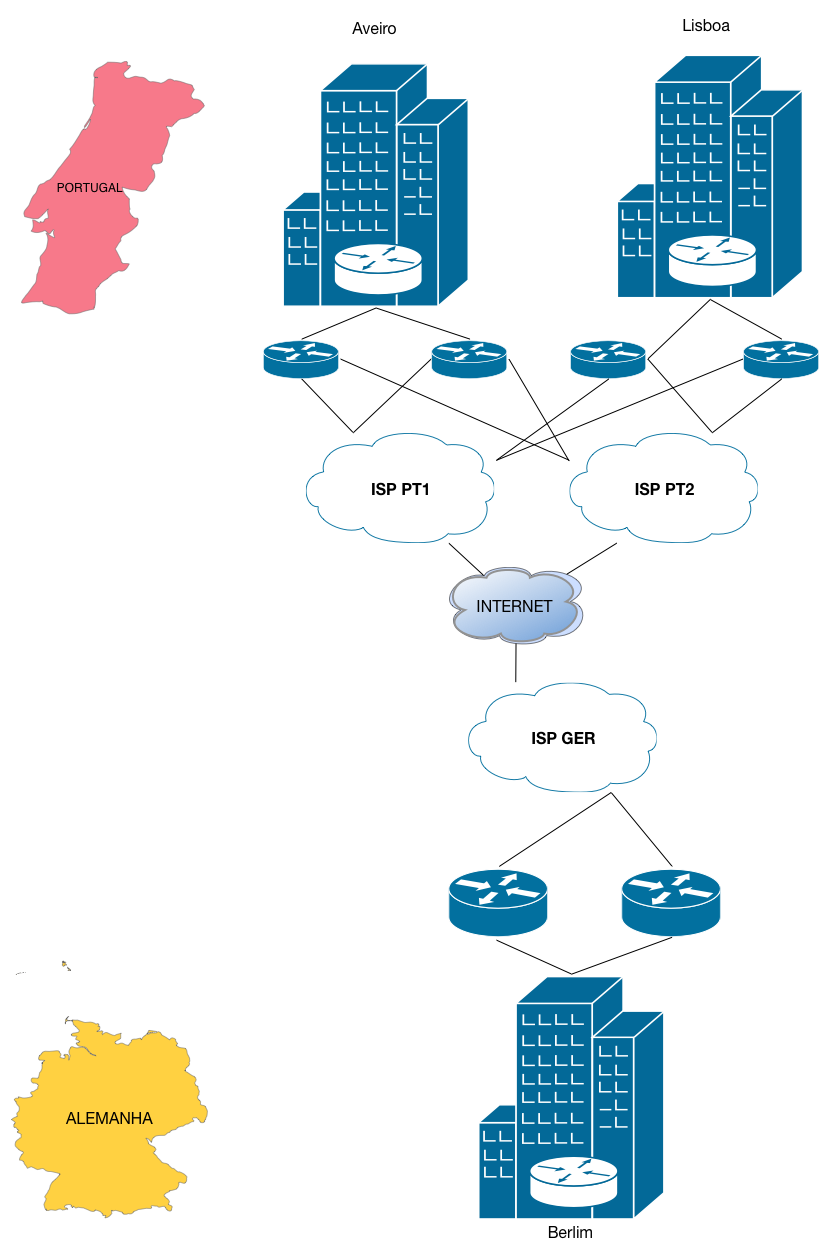
\includegraphics[width=100mm]{visao_global.png}
\end{figure}

\newpage

	A empresa XYZ, Inc. possui dois contratos de acesso à Internet com dois ISP portugueses (ISP PT1 e ISP PT2) para os edifícios de Aveiro e Lisboa. Possui também um contrato com um ISP alemão (ISP GER), para o edifício que se situa em Berlim.
	
	A empresa adquiriu as redes IPv4, 193.10.10.0/24 e 196.1.1.0/26, em Portugal e na Alemanha, respectivamente. Também adquiriu as redes IPv6 2002:C:C::/48, em Portugal e 2001:F:F::/48 na Alemanha.
	
	De forma a poupar endereços públicos IPv4, cuja totalidade não seria suficiente para todos os terminais, serão utilizadas redes privadas NAT em cada edifício. A atribuição de endereços privados IPv4 será efectuada segundo a seguinte forma 10.EDIFICIO.VLAN.Host/24  e de endereços públicos IPv6 2002:C:C:EDIFICIOVLAN::Host/48 em Portugal e 2001:F:F:EDIFICIOVLAN::Host/48 na Alemanha, onde (EDIFÍCIO = número que identifica o edifício e VLAN = número que indica a VLAN). Temos que:
	
	TABELAS
	
	Como é possível observar nas tabelas acima, apenas as VLAN’s 1 e 10 (Administração e Wireless) são End-to-End, que podem ser utilizadas nos vários edifícios. As restantes VLAN’s serão Locais, só estarão disponíveis no próprio piso. A utilização de QoS (Quality of Service) é potenciada, pois a cada VLAN está associado um serviço diferente.

	No edifício de Aveiro, por exemplo,  a VLAN 3 terá endereços IP do tipo 10.1.3.HOST/24.	
	A regra referida acima não será utilizada pelas VLAN’s 6, 8 e 12 pois possuem endereços IP públicos já atribuídos.




\end{document}
